\chapter{CERN Web Landscape}
\label{cern_web_landscape}
In this chapter I am going to blahblah about CERN web landscape obviously
\thispagestyle{empty}


\section{Current Relevant Tools}
\subsection{WAP or WAD}
\subsubsection{Wappalyzer}


\section{Travaux de Simon Henein}
\subsection{Conception des guidages flexibles}

\begin{figure}[!ht]
\centering
%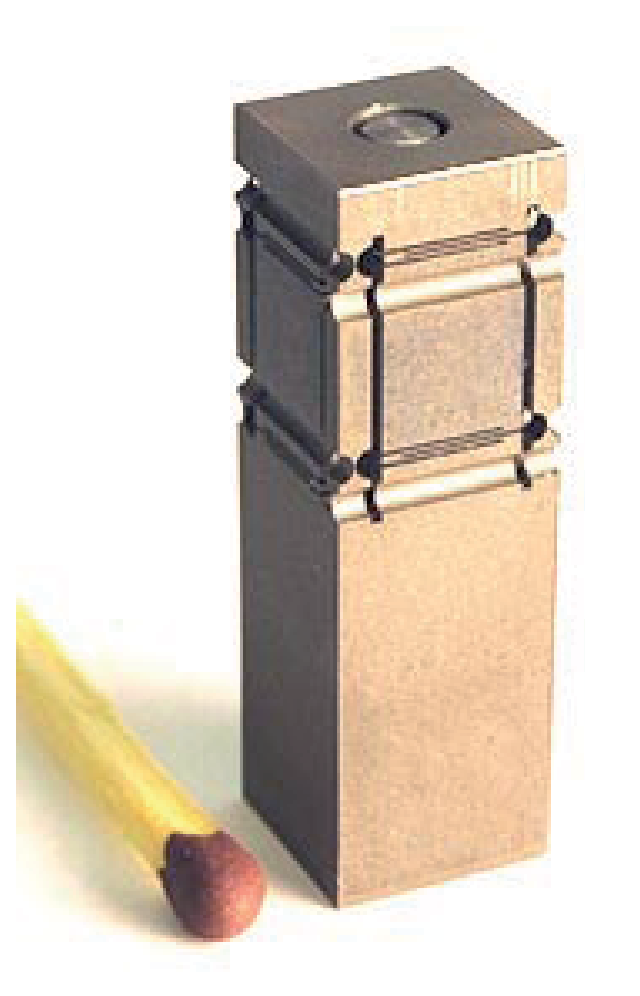
\includegraphics[width=3cm]{figure1.eps}
\caption{figure caption}
\label{fig: image_pivot_fex}
\end{figure}

\newpage

in a new page now
\begin{itemize}
\item first item
\item second item
\item third item
\item fourth item
\end{itemize}

\noindent no indent??


\subsection{Flexure pivot for aerospace mechanisms \cite{henein}}


\begin{figure}[!ht]
\centering
%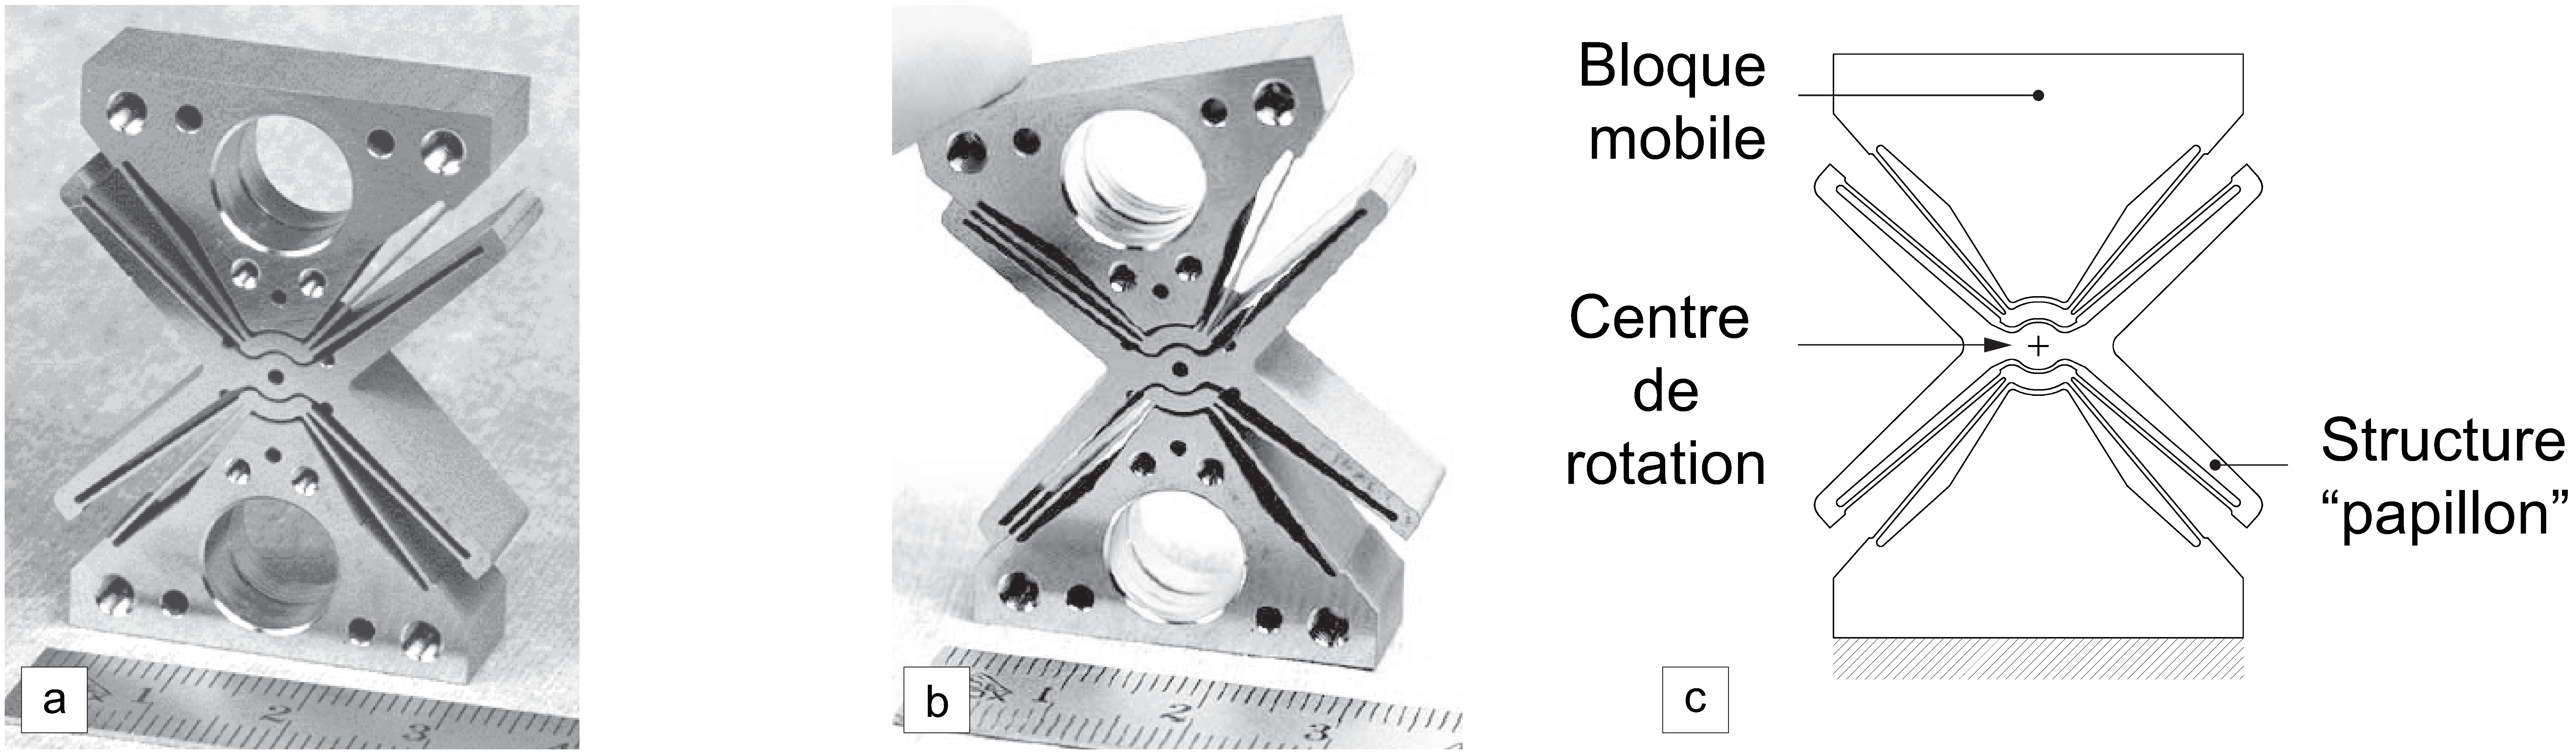
\includegraphics[width=12cm]{figure2.eps}
\caption{Guidage flexible: (a) pivot papillon \ (b) pivot papillon sous contrainte \ (c) something else}
\label{fig: mix_pivot_pap}
\end{figure}

\noindent adasd
\begin{figure}[!ht]
\centering
%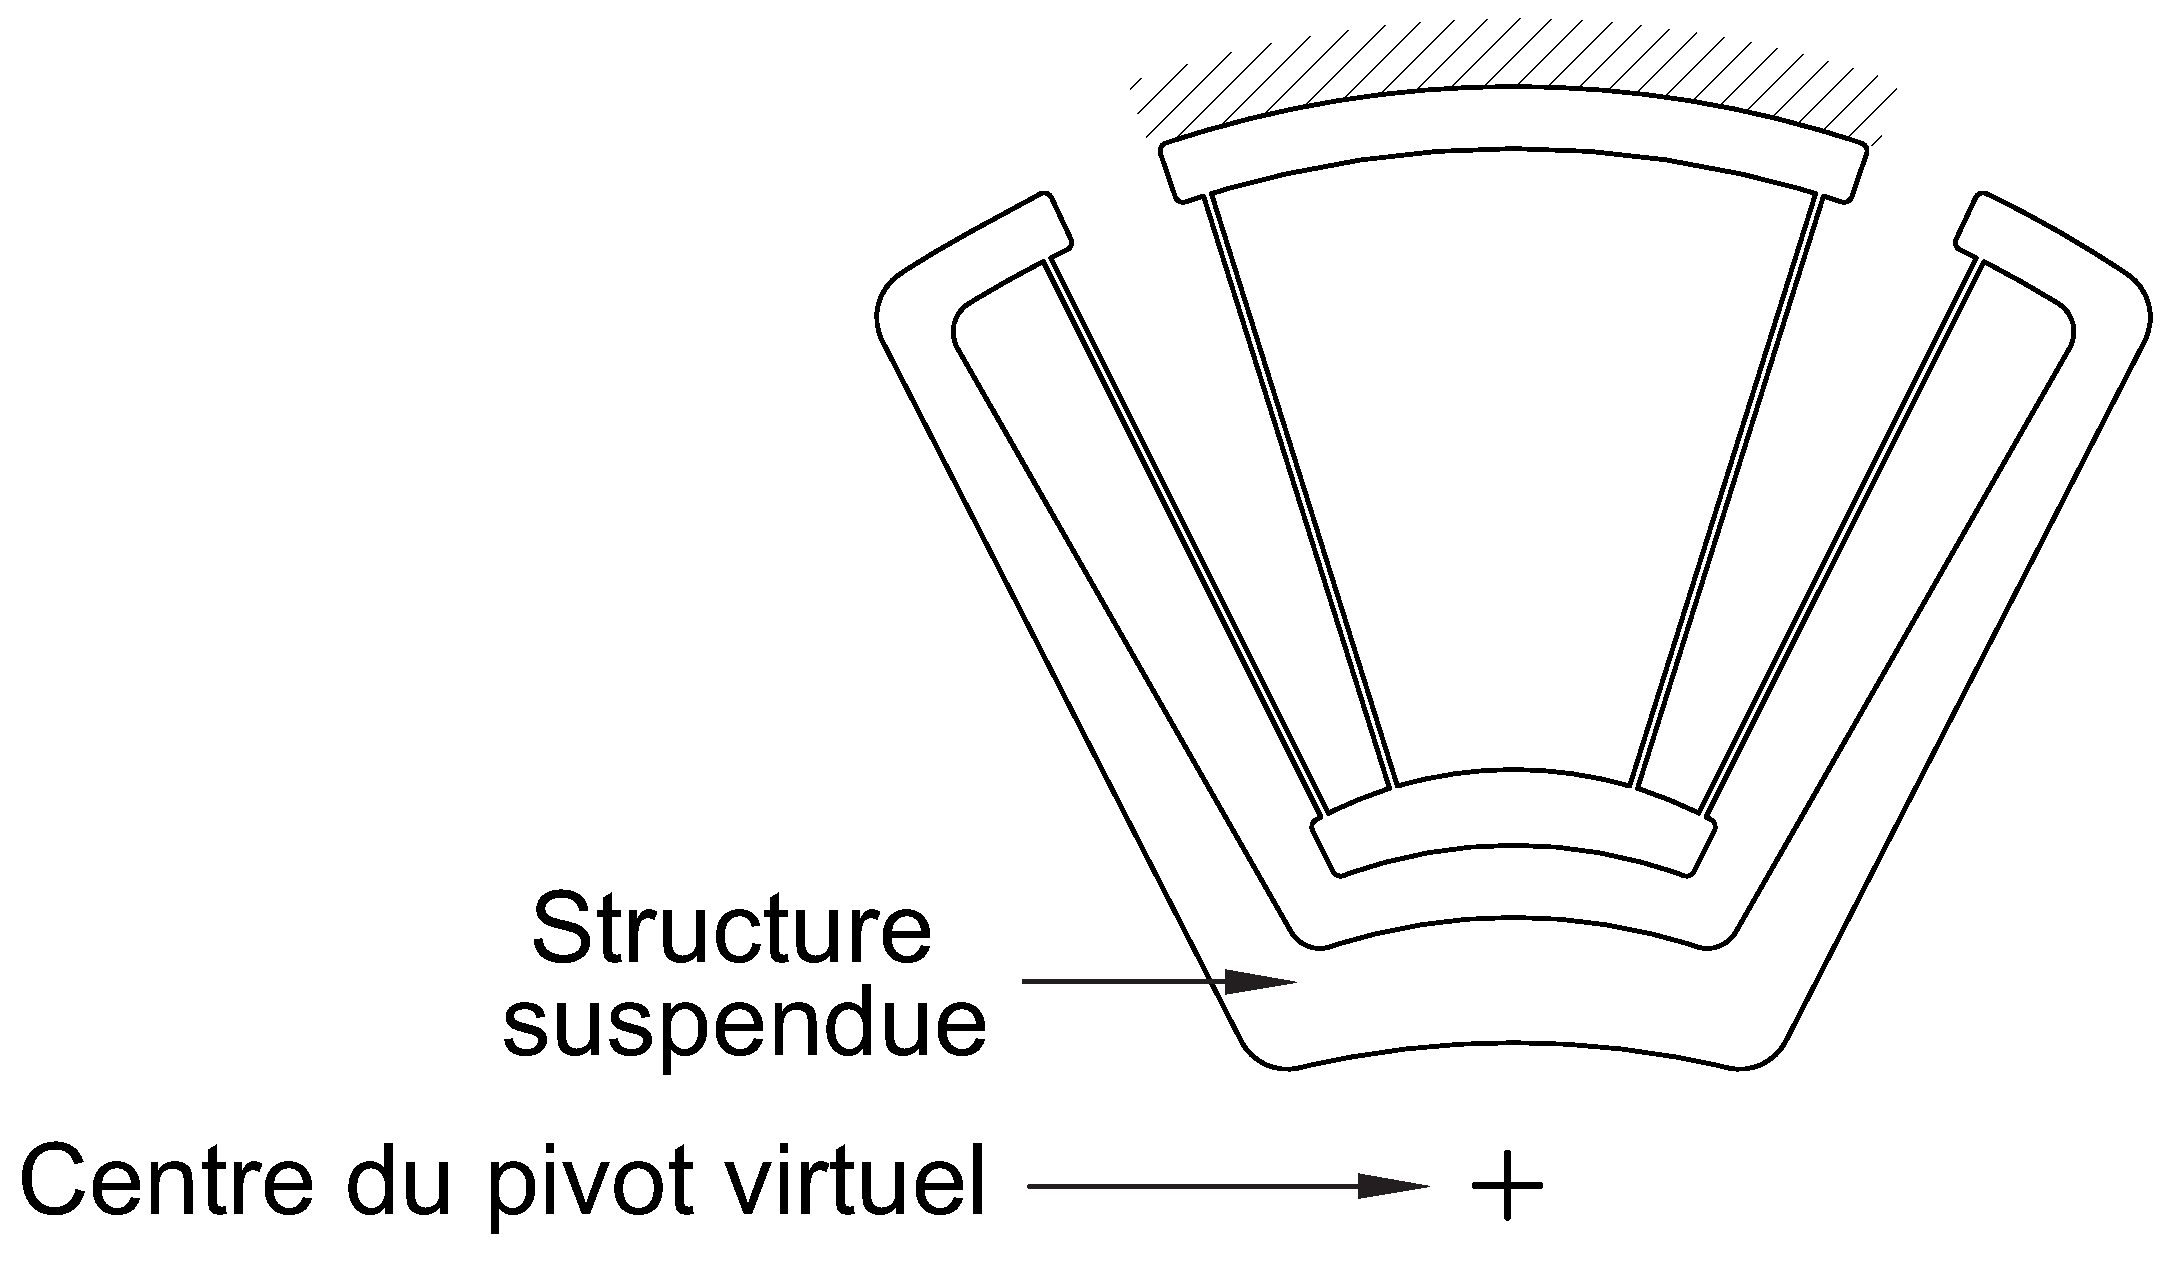
\includegraphics[width=6cm]{figure3.eps}
\caption{Pivot flexible: structure et centre de rotation}
\label{fig: schema_pivot_flexible_art}
\end{figure}




\section{Three-Phase Electrostatic Rotary Stepper Micromotor with a Flexural Pivot Bearing \cite{confidential}}


\begin{figure}[!ht]
\centering
%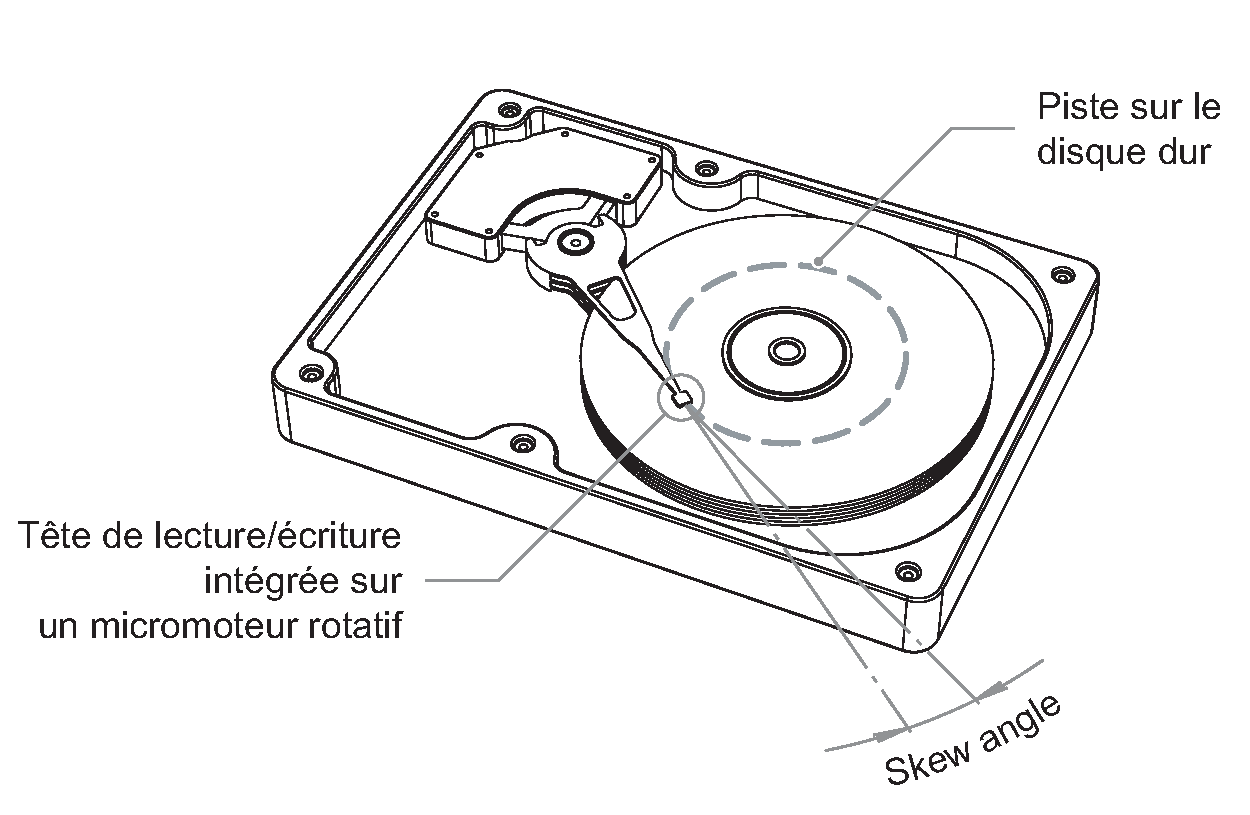
\includegraphics[width=8.5cm]{figure4.eps}
\caption{Disque dur: "skew angle" entre la piste et la t�te de lecture}
\label{fig: schema_HDD}
\end{figure}

\begin{figure}[!ht]
\centering
%\includegraphics[width=12cm]{figure5.eps}
\caption{Moteur:(a) moteur monolithique \ (b) asdasd}
\label{fig: image_moteur_JMEMS}
\end{figure}


\noindent asas
\label{improvements}
\begin{itemize}
\item sdf
\item sdf
\item dsf
\end{itemize}

\noindent sdfsdf

\newpage










\section{Single mask 3-phase electrostatic rotary stepper micromotor \cite{transducers}}


\begin{figure}[!ht]
\centering
%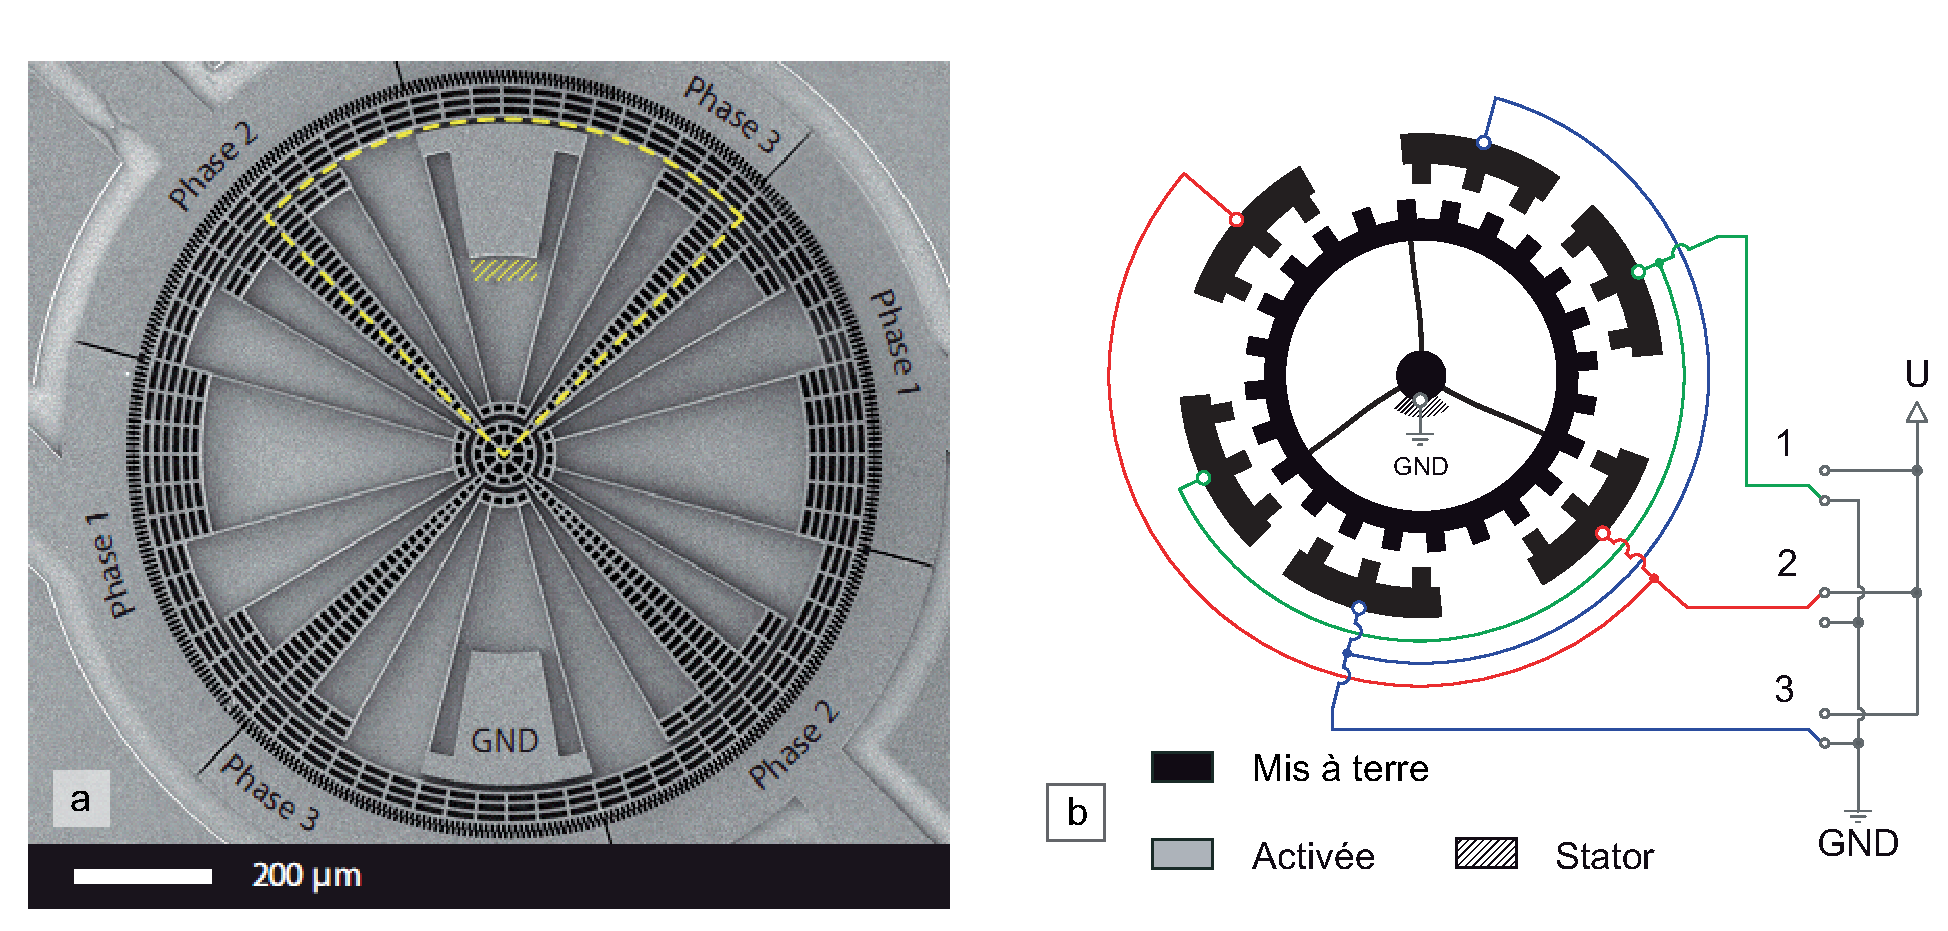
\includegraphics[width=12cm]{figure6.eps}
\caption{Moteur: (a)  moteur monolithique \ (b) asdsad}
\label{fig: image_moteur_edin}
\end{figure}

It's supposed to be funny! 






